\chapter{Discussion}\label{ch:Discussion}\addtocontents{lof}{\protect\contentsline{chapter}{\protect\numberline{\thechapter}Discussion}{}{}}
\newthought{Synopsis}\synopsisDiscussion

\section{Challenges and the Various Explored Approaches}
\subsection{Modelling Challenges}
\newthought{Mould Die Design}\\
The challenges in the early stages after deciding to work off of an pre-constructed anatomic valve geometry spawned many issues, it didn't allow for feature interaction in SolidWorks which prompted some very suboptimal prototyping choices that ended in a huge amount of time investment for an avenue that was eventually made obselete upon later findings. The series of 2-stage epoxy moulds developed as discussed in \cref{fig:moulddie} had a 72 hour curing time, which made the turnaround for learnings much slower to implement.

This process became obselete when the SolidWorks package being used was arbitrarily updated. It was discovered that the 'Segment Mesh' tool previously attempted to use to convert the STL to mesh body and then to a solid part had been overhauled to allow more complex geometries to be segmented. On this discovery the part was successfully converted to a solid body which allowed for it to be subtracted from an encompassing cylindrical body as originally theorised which was then split into the what were the foundations of the final design press mould pieces.

From this point further iterations of the press mould were much quicker, taking only 4-5 hours, reducing the print-to-casting time by 95\%. 20 hours for finalised designed where the layer lines were much smoother, being almost invisible on the casted part.
\begin{figure}[H]
    \centering
    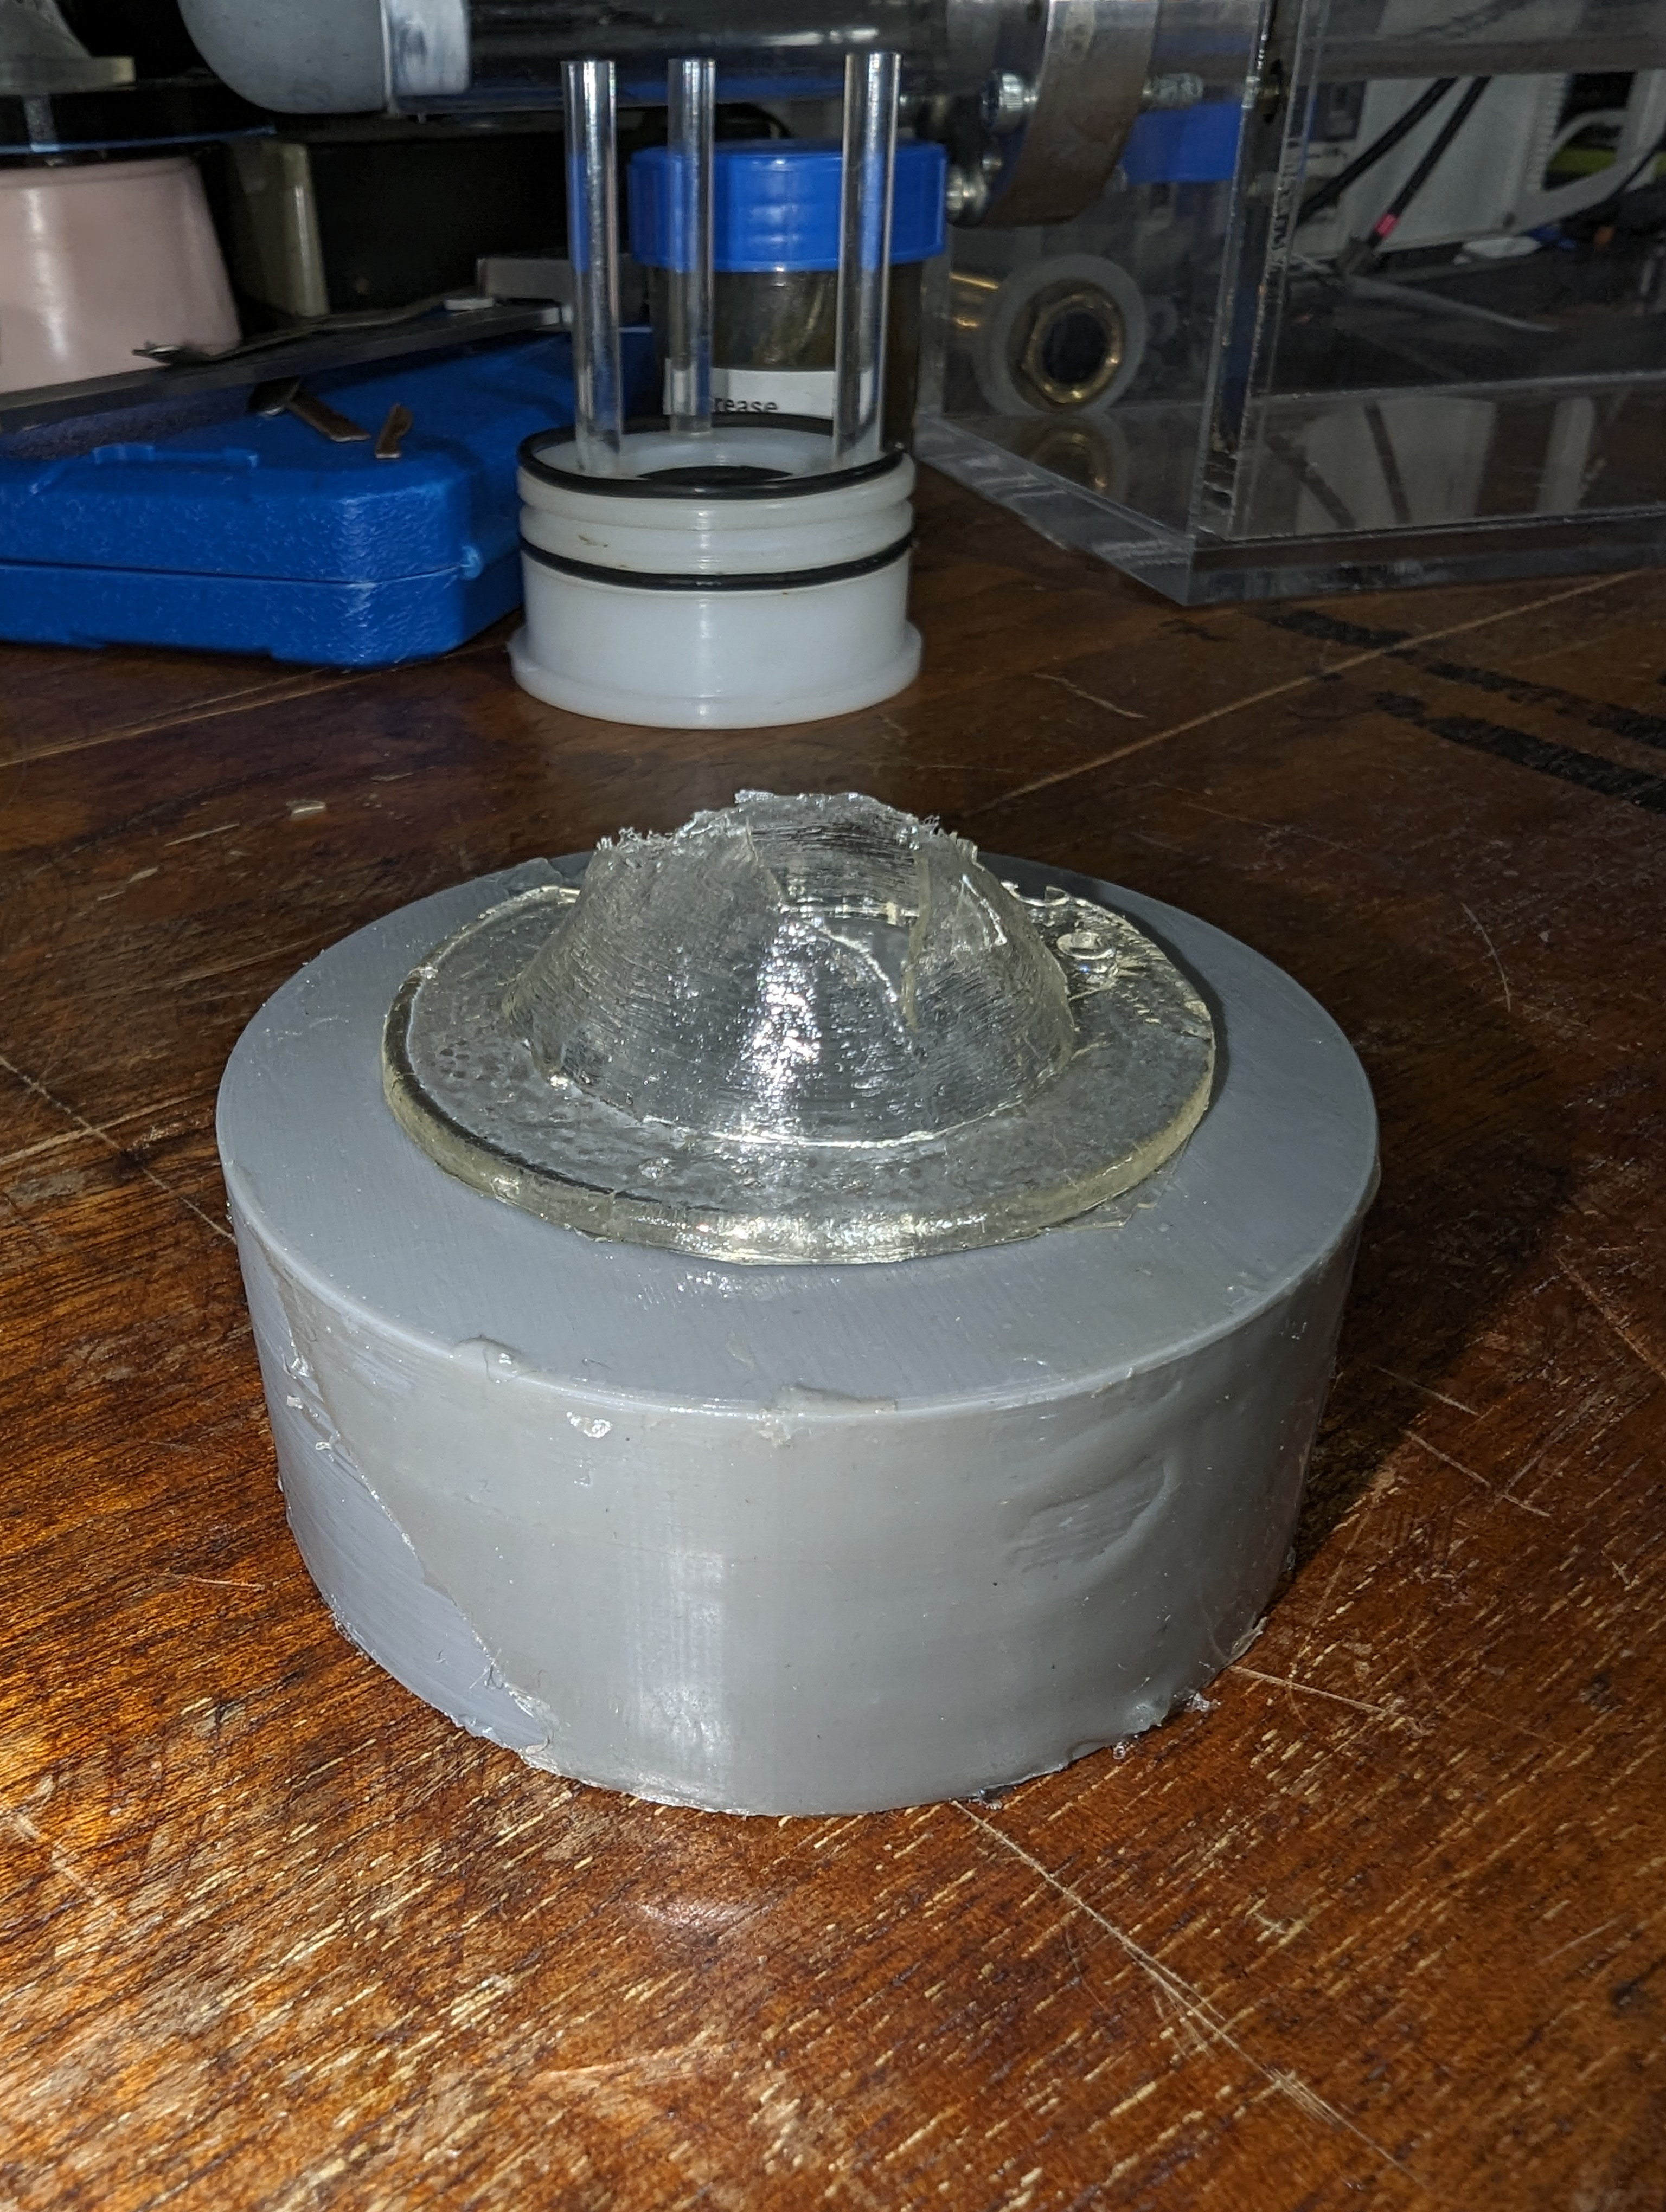
\includegraphics[width=0.75\textwidth]{figures/latercastnice.jpg}
    \caption{Final cast of anatomical valve}
    \label{fig:cast1}
\end{figure}

\newthought{Valve Design}\\
Another area that caused an excess of time used was the post processing of the anatomical valve geometry, in becoming acquainted with STL modelling\sidenote{Software packages like blender use mainly sculpting tools that are used to modify the surface as opposed traditional CAD programs like SolidWorks where parts are built up from a tree of features} on the various programs trialed throughout the study the model was transferred across systems a lot to utilize the different tools each had, for example, how blender had great scuplting tools but lacked simple geometry analysis which was required for monitoring the surface as the thickness was homogenised.

While blender has capabilities to manipulate shaders to render this kind of information however due to it being an opensource program the process of developing a custom shader for this purpose was deemed too rescource intensive however if further work was conducted with many patient-specific models being developed it would be quite likely the most efficient option.

\subsection{Manufacturing Challenges}

\newthought{Chordae Tendineae Prototyping}\\
The tendineae attachment to the leaflets was another highly contested and thought out factor of the design. Balancing the rigidity that is added to the leaflets by some methods in attaching the nylon wire and the adhesion to the leaflet is very dificult, for the scope of this study it was found that B7000 adhesive worked well as the tendineae could be effectively attached with minimal disruption to the mechanics of the valve however this did add thickness to the leaflets which not only adds rigidity that hinders coaptation in experimental use but also brings many issues for potential computational simulations that could be conducted in tandem to a study of this nature.

Studies like \citeonly{karlExvivoInvitroDynamic2024} which had been examined in the later stages of the study use a method of embedding their chordae tendineae within the leaflets, containing a medical gauze matrix, so that the tendineae do not detach under tensile forces. An approach like this could prove very effective in application to this study as it would simplify the manufacturing process in that with a the tendineae can be attached to the gauze matrix prior to \gls{PU} casting ensuring accurate and replicable placement.

\newthought{Valve Prototyping}\\
The prototyping conducted through the study for the mould parts, fixturing and experimental rig revealed a few key insights into the rapid-prototyping landscape. For each print the configuration of the printer was tailored to the purpose of the parts being produced, parts being made in early iterations were set to a faster infill and layer height setting, whereas finalised ideas were set to slower, higher resolution settings.

It was found these dense high definition settings needed for aaccurate and rigid mould die had issues of their which took many iterations and failed prints to perfect. They often resulted in a large amount of stringing, a printing defect, which in many cases was not solvable via post processing. To circumnavigate this the researchers in the UCD print lab were consulted. Tailored settings in Prusa Slicer were then programmed for the geometry where the resulting gcode would stop the nozzle from crossing the perimeter of the valve moulds, retraction settings would stop the printer from leaving blobs of plastic on the interior of the mould and z-axis seams were alligned to not interfere with the geometry.
\mynewline
In earlier stages of the study a resin \gls{SLA} printer was used to manufacture an anatomic model for the silicone mould method discussed in \cref{fig:silimould} which however it was not feasible to develop further iterations from resin due to the printer being in a separate lab and having a much higher cost of with proprietary resins. Two major benefits to \gls{SLA} printing are;

\begin{figure}[H]
    \centering
    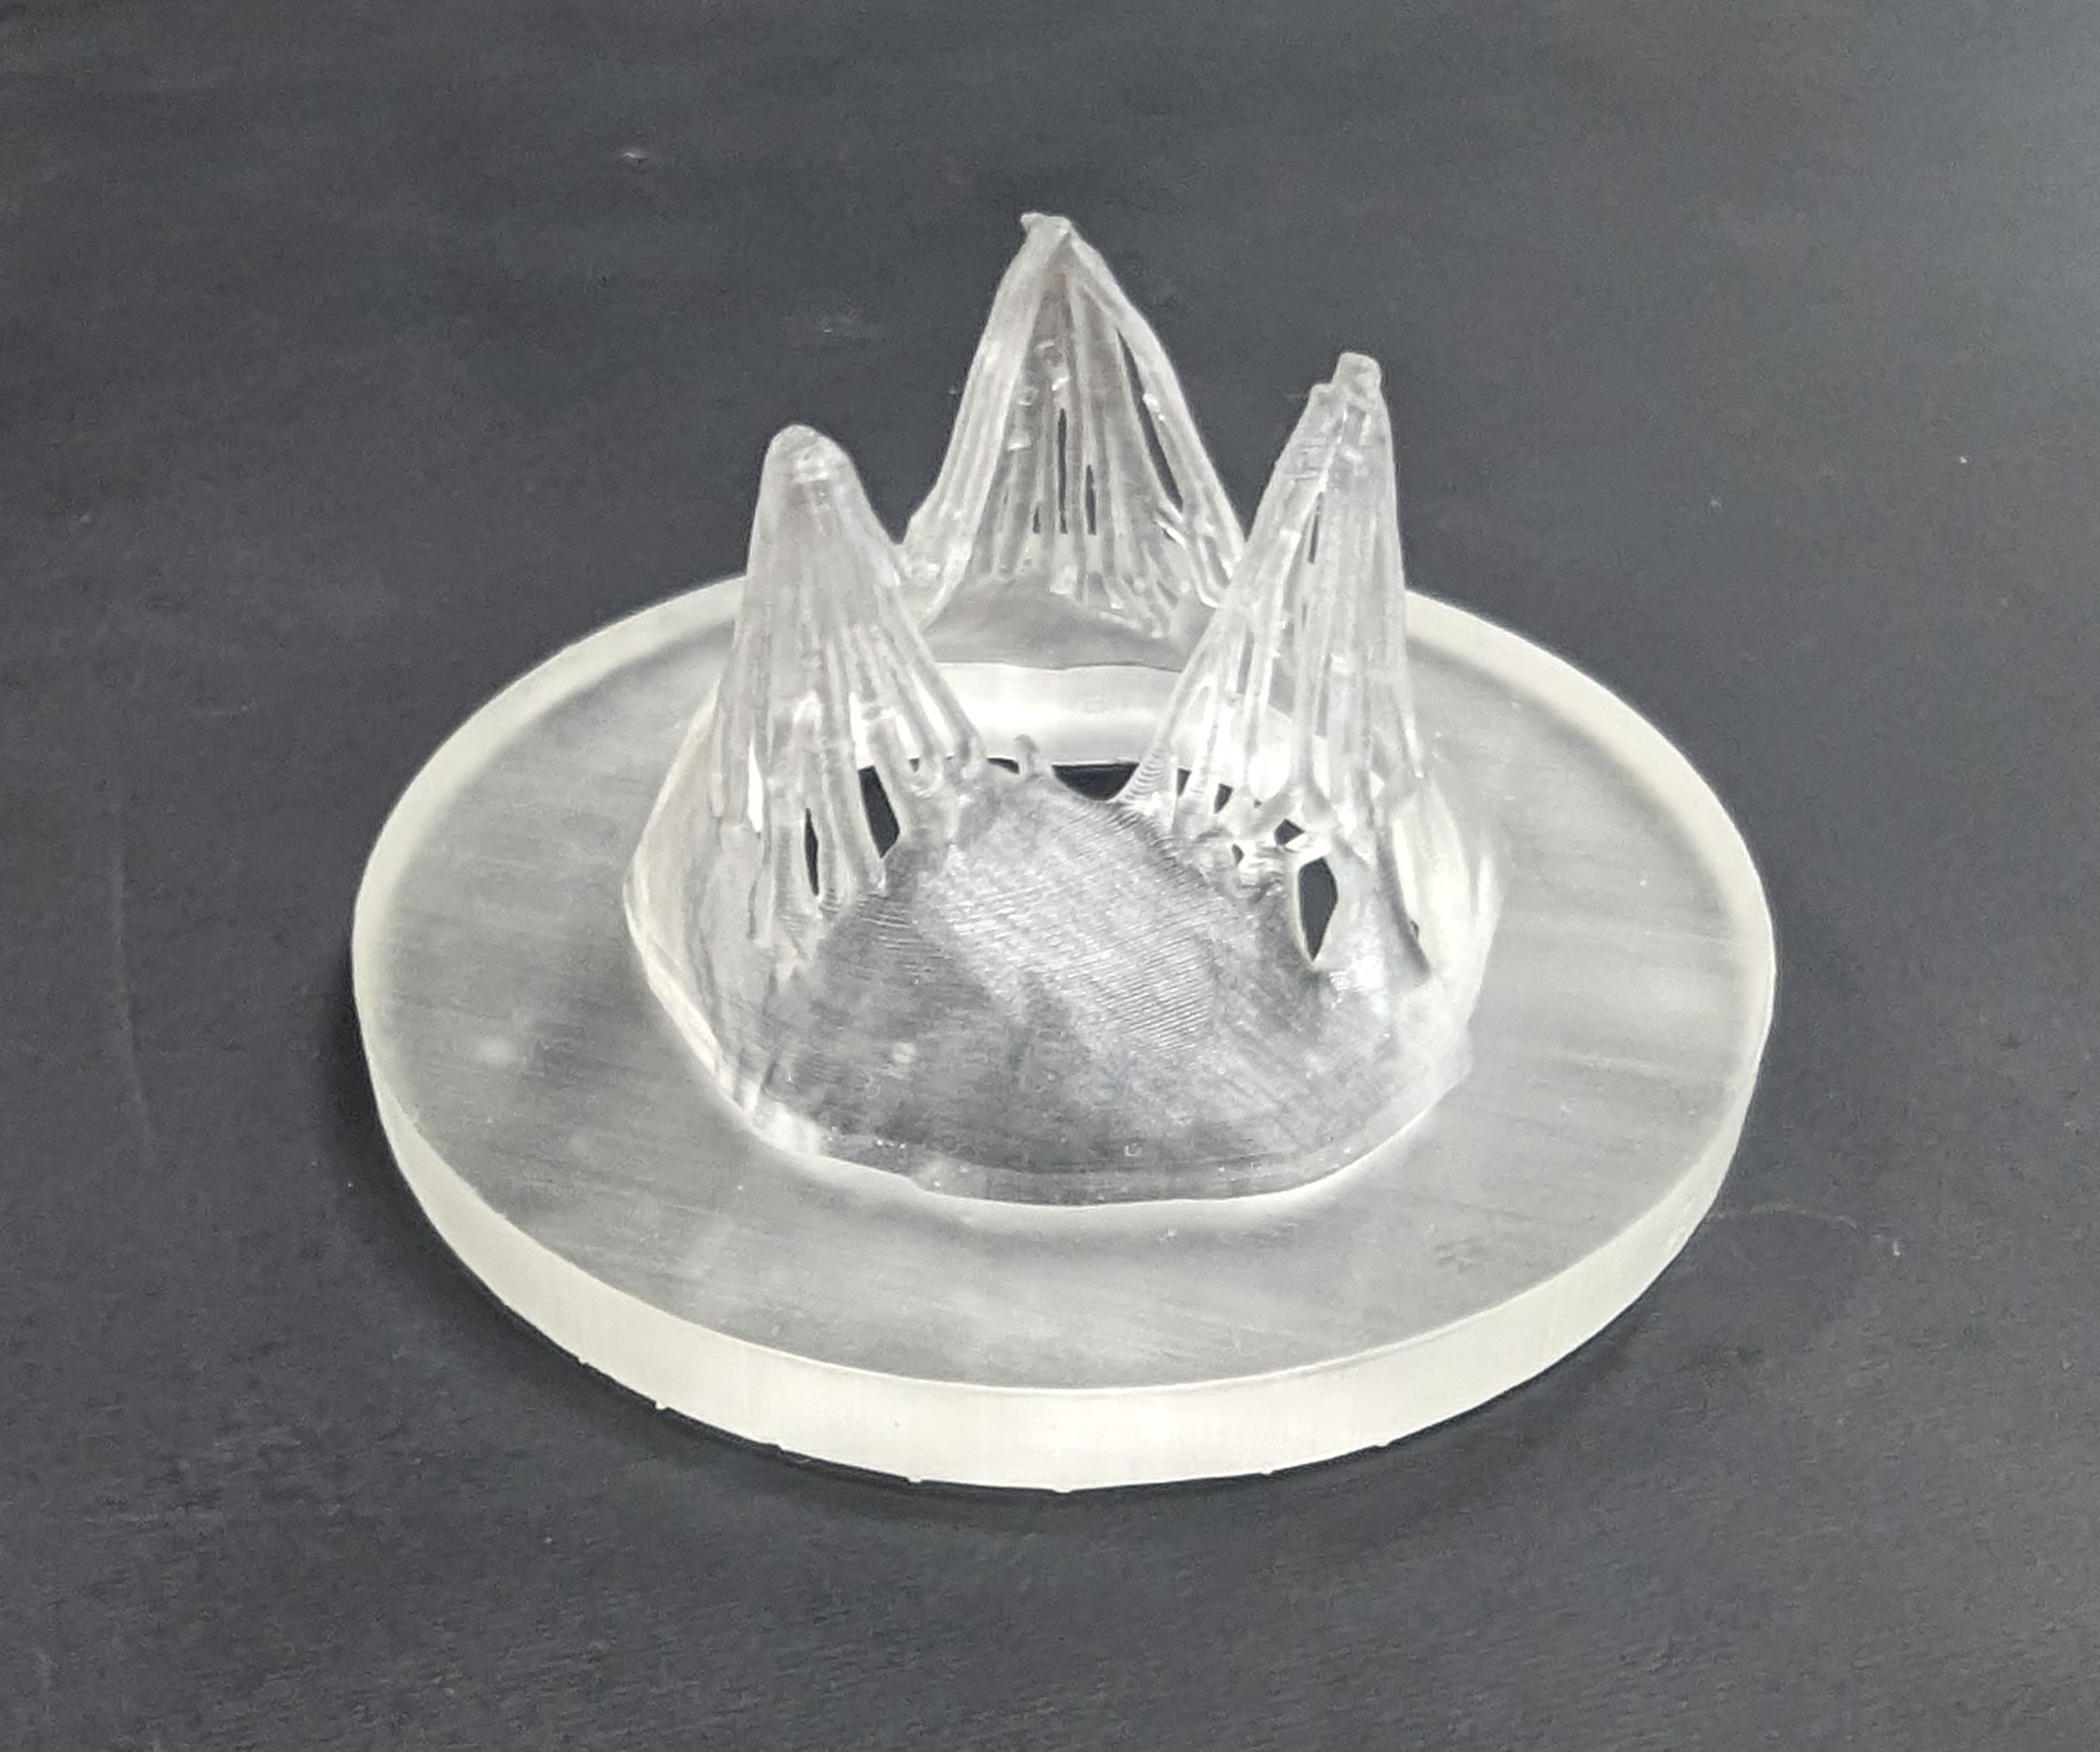
\includegraphics[width=0.75\textwidth]{figures/resinprintanat.jpg}
    \caption{Early revision \gls{SLA} print of anatomical valve}
    \label{fig:reso}
\end{figure}
\marginpar{\textbf{Resources:}
    \begin{itemize}
        \item \href{https://help.prusa3d.com/article/faq-frequently-asked-questions_1932}{Prusa TDS}
        \item \href{https://formlabs.com/blog/understanding-accuracy-precision-tolerance-in-3d-printing/}{FormLabs TDS}
    \end{itemize}
}
\begin{itemize}
    \item The vastly increased tolerance of resin printing\\
          Prusa \gls{FDM}:0.3mm\\
          FormLabs \gls{SLA}:0.01mm
    \item The reduced layer height that resin printing is capable of\\
          Prusa \gls{FDM}:0.05mm\\
          FormLabs \gls{SLA}:0.025mm
\end{itemize}
This has two main benefits regarding this study;
\begin{itemize}
    \item Minimizing layer height results in mould parts reduces surface affects
    \item Reducing adhesion of cast part to mould, this is minimized on \gls{PLA} parts with mould release and sanding however with casted parts on this degree of thickness there can still be an increased risk of breakage in the demoulding process.
\end{itemize}
Another option worth considering is machining from either steel or a performance plastic like delrin \citeonly{liProcessOptimizationInmold2022}, this would be more expensive however it could be worth the cost for moulds that need to be used for a larger number of castings as well as increasing the precision over multiple casts since you the 3D printed parts can warp under the pressure of the clamping. The transparency of the part was a consideration for further work on the valve as the proposed integration into the right heart simulator would involve \gls{PIV} measurement where maintaining transparency would allow for an measured flow field uninterrupted by the valve, this was an issue in studies like \citeonly{rabbahNovelLeftHeart2013} and the efficacy on dynamic transparent parts in \gls{PIV} rigs has been shown in studies like \citeonly{busenDevelopmentVitroPIV2017}

\section{Contextualizing Results}

% Discuss how your results relate to previous studies and theoretical frameworks. Are your findings consistent with other studies, or do they diverge?
% Analyze the significance of any discrepancies and explore possible reasons.

The results of this study have shown how development of imitative synthetic heart valves can be a valuable tool in cardiac simulators. The coaptation tests on the valve show great promise for technology of this nature, previously in simulational studies such as \citeonly{rabbahNovelLeftHeart2013} dissected porcine valves, \citeonly{gintyModelingPatientSpecificDeformable2018} used rigid valves and \citeonly{raghavExperimentalAssessmentFlow2018} non-anatomically representative valves which each have major limitations in their ability for a wider range of experiments.\\
Some such limitations of these valves which the work of this study has surpassed are;
\begin{itemize}
    \item The longevity of porcine for repeated experiments. While it can be stored in the likes of formalin the tissue degrades over time which leads to an irrepeatability in testing and eventual need for replacement.
    \item Semi-rigid valves can't be used in flow studies as they can't deform to coapt.
    \item Non-anatomical valves can coapt but don't represent true geometry which won't yield accurate results.
\end{itemize}

\newthought{Chordae Tendineae Performacnce:}\\
The coaptation test illustrated how the chordae tendineae can be used in a synthetic part to prevent prolapse and aid coaptation. The aligns well with how it had been done before such as in \citeonly{rabbahNovelLeftHeart2013} and \citeonly{karlExvivoInvitroDynamic2024} where native and synthetic tendineae were used respectively. Such works also show how this part of the model can be manipulated with motors to simulate the contraction of papillary muscles which while not applicable to the current design of the right heart simulator, could be developed for future iterations or simpler rig design like that of the tube-based coaptation test \cref{fig:Videos}

\newthought{Leaflet Performance:}\\
The area with most room for improvement is likely the leaflets. The final iteration from this study came very far relative to the initial iterations in term of rigity, transparency and geometrical precision, it also performed better than similar attempts from other studies like \citeonly{gintyModelingPatientSpecificDeformable2018} although in regards to the initial design criteria from section:\cref{sec:Design Criteria}  it is lacking in functional performance and scalability

Not all the leaflets coapted together which was the objective however it was supposed to occur from annulur dilation and chordal loosening not from just the geometry, this is most likely due to the model of the valve being based off a valve in the diastolic phase so the full length of the leaflets was malformed in \gls{CT} conversion as they weren't not being under load from the presuure. This can be seen in \cref{fig:Videos}:B where the leaflets do move back but are not long enough to meet eachother. The work of \citeonly{karlExvivoInvitroDynamic2024} capture this well in their mitral valve design, they did well with leaflet length however theyre design was not anatomically representative, building off this to capture both physiological replicity and functional performance would be a first of it's kind for in-vitro tricuspid valve testing.




